Three different prototypes has been developed in the framework of the tritium project for detection of tritium activities in the water which is used by Nuclear Power Plants. In each detector several improvements has been included in order to increase their efficiency and reduce the LDL (Low Detection Level) of tritium. 

The table \ref{} summarize the most important parameters of each prototypes.

TABLE

CONCLUSIONS

The next step will be to install in arrocampo nuclear power plant three detectors like Tritium-IFIC 2, which we will call cells. 

The cells are essentially the same as the prototype. These have minimal differences which are necessary to work in Arrocampo since the water needs to flow through the cells. In the picture \ref{fig:Cell_prototype} we can see both, a Tritium-IFIC 2  prototype and one cell. 

\begin{figure}[htb]
\centering
{
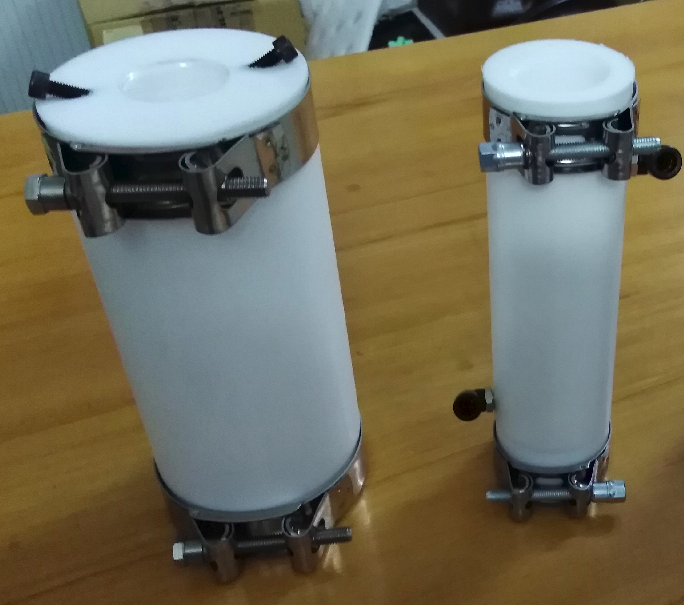
\includegraphics[scale=0.25]{Cell_Tritium_IFIC_2.png} 
}
\caption{Tritium-IFIC 2 prototype in the left size and Cell of Tritium detector in the right side \label{fig:Cell_prototype}}
\end{figure} 


There we can see that the cells are thinner than the Tritium-IFIC 2 prototype. This is because we don't need the holes in the top of the detector, whose function is to fill the prototype. Instead of that, water will flow continuously through the cells so we need two pieces in the cells (black pieces) from where the water will enter to the cell, it will cross the fibers and it will leave the cell. All these differences are little modifications which souldn't affect the the detector efficiency.

First we will install three identical cells that we will read in parallel. With this parallel reading we won't improve its efficiency, it will only be maintained, but we will reduce their LDL which is very important because the activity which we want to detect follow the ALARA principle (As Low As Possible Achievable). If it is necessary we can install more cells that we can read in parallel, as many as we need for arriving to our objective, $100~\becquerel/\liter$